\chapter{Hierarchical Clustering of LC-MS Peaks}
\label{c:hdp}

\section{Introduction}

The Cluster-Cluster method introduced in Chapter~\ref{c:precursor-clustering} performs the direct-matching of peaks in ionisation product (IP) clusters that themselves have been clustered together. However, related peaks are assigned into IP clusters based on their \textit{maximum a-posteriori} probabilities. In this chapter, we expand upon the idea of alignment as a hierarchical clustering problem by proposing \textbf{HDP-Align}, a Bayesian non-parametric model that groups related peaks within runs by their retention time (RT) and assigns them to global clusters shared across runs. Within each global cluster, peaks are further grouped by their m/z values into mass clusters, representing the various ionisation products derived from the global compound. In this manner, the local clusters in HDP-Align correspond to the within-file IP clusters from running PrecursorCluster on each run, while the global clusters in HDP-Align correspond to the top-level clusters produced from Cluster-Cluster (described in Chapter~\ref{c:precursor-clustering}). 

The proposed HDP-Align model introduced in this chapter allows us to infer the matching of peaks across all runs at once without the need for any intermediate merging of pairwise runs. Similar to the Cluster-Cluster model introduced in Section~\ref{sub:cluster-match}, the proposed model of HDP-Align also introduces the possibility of allowing the user to trade recall for precision from the alignment results by returning a smaller subset of the results having a higher confidence score of being correctly aligned. Figure \ref{fig-hdp-cartoon} shows an illustration of the clustering process in HDP-Align. Additionally, the latent variables inferred in the model may correspond to chemically meaningful compounds and can be used for further analysis. Using a metabolomic dataset, we demonstrate the usefulness of such latent objects by using the mass clusters derived from the model and a set of defined ionisation product transformations to perform the putative annotations of peaks based on their potential adduct types and metabolite identities.

\begin{figure}[!htbp]
\centering\includegraphics[width=0.50\linewidth]{06-hdp/figures/figure_1.eps}
\centering\caption[An illustrative example of how the proposed model in HDP-Align works.]{An illustrative example of how the proposed model in HDP-Align simultaneously \textbf{(1)} performs the clustering of related peaks into within-run local clusters by their RT values, \textbf{(2)} assigns the peaks to global \ac{RT} clusters shared across runs, and \textbf{(3)} separates peaks into mass clusters, which correspond to aligned peaksets.\label{fig-hdp-cartoon}}
\end{figure}

\section{Related Work}

The goal of establishing the matching of peaks across multiple runs at once can be viewed as a clustering problem, where a set of peaks can be grouped (by their m/z, RT and other suitable features) into local clusters within each run (representing all of the peaks from an individual compound), which are further grouped into global clusters shared across runs. Hierarchical clustering has been used for the matching of peaks across runs \cite{Tibshirani2004, DeSouza2006}. In \cite{Tibshirani2004}, peaks are hierarchically clustered based on their m/z values to construct matching across runs, while in \cite{DeSouza2006}, peaks from the entire dataset are pooled and a hierarchical clustering scheme based on RT only is used to group peaks into within-run local clusters, which are further grouped into across-run super clusters. Both approaches require choosing various user-defined parameters, such as determining a suitable cut-off for the dendogram produced, deciding on a suitable linkage method and defining an appropriate distance measure between groups of peaks. In \cite{Tibshirani2004}, no chromatographic separation is performed, so only the m/z values of peaks are used. The nature of the gas chromatography data used in \cite{DeSouza2006}, where retention time across runs is more reproducible, means that even without using the m/z information, good alignment performance can still be obtained. This will not be the case of LC-MS data, where retention time drift is common and the highly accurate m/z information is crucial for alignment. The proposed HDP-Align model fills this gap where both m/z and RT values, important for LC-MS peak alignment, are used for the hierarchical clustering process. The probabilistic approach employed by HDP-Align also allows us to extract confidence values from aligned peaksets.

\section{Hierarchical Dirichlet Process Mixture Model for Alignment}

The proposed model for HDP-Align is framed as a Hierarchical Dirichlet Process (HDP) mixture model \cite{teh2012hierarchical}. Essential modifications to the basic HDP model, described in Section~\ref{background-hdp-clustering}, were performed to suit the nature of the multiple peak alignment problem. Figure \ref{fig-platediagram} shows the conditional dependencies between random variables in the HDP-Align model.

\begin{figure}[!htbp]
\centering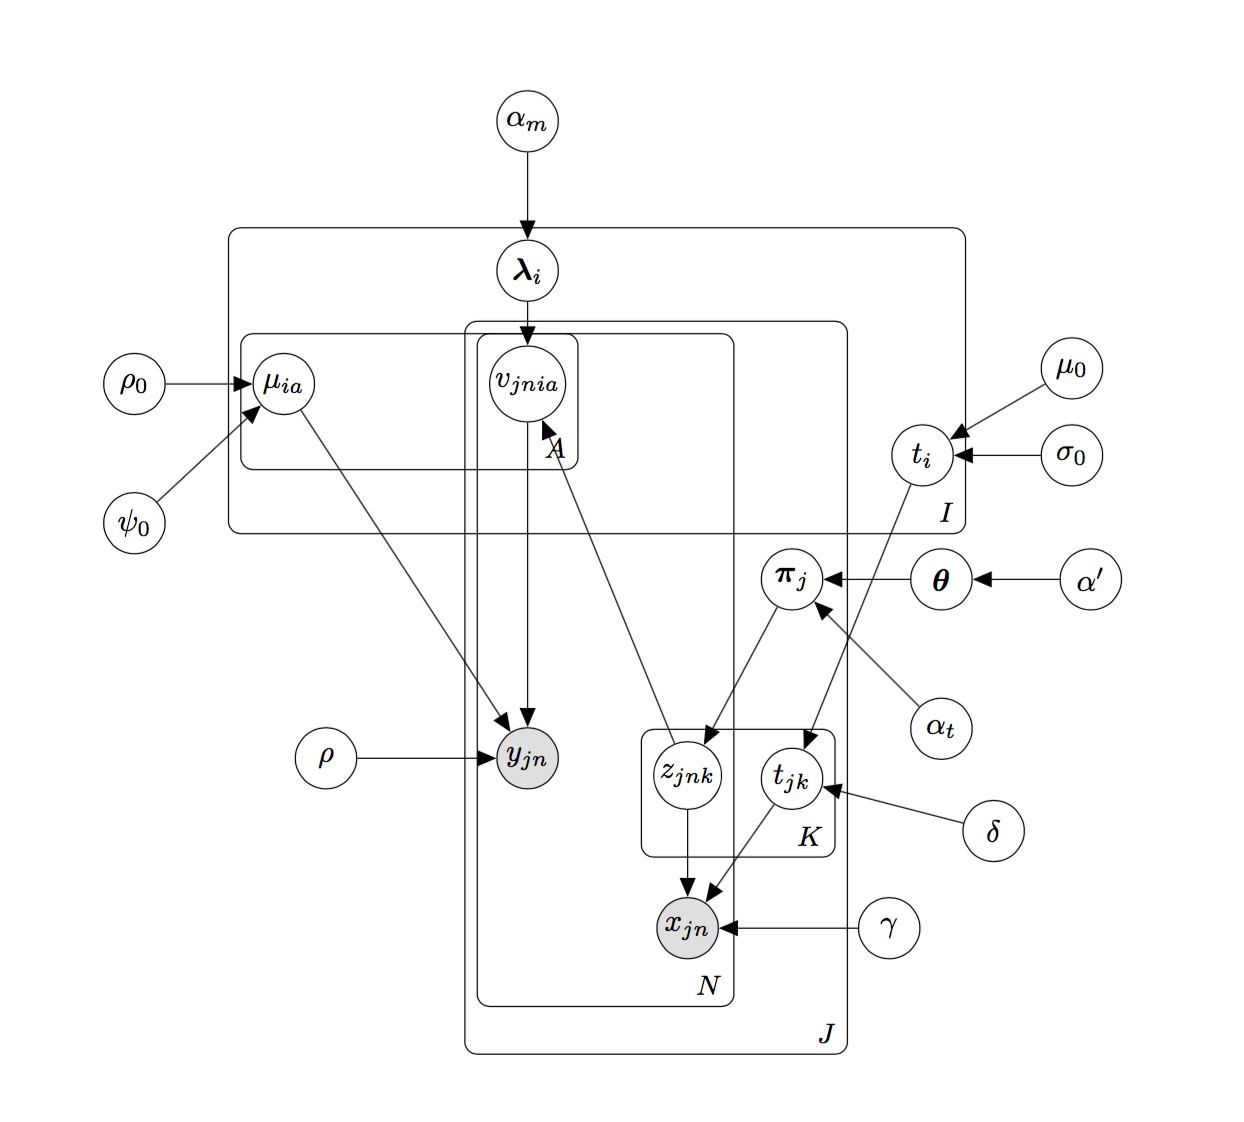
\includegraphics[width=0.9\linewidth]{06-hdp/figures/model_hdp.png}
\centering\caption{Graphical model for HDP-Align. $x_{jn}$ is the observed RT value of peak $n$ in file $j$, while $y_{jn}$ is the observed m/z value.\label{fig-platediagram}}
\end{figure}

Our input consists of $J$ input files, indexed by $j=1,...,J$, corresponding to the $J$ LC-MS runs to be aligned. Each $j$-th input file contains $N_j$ peaks in total, which can be separated into $K_j$ local clusters of related-peaks. In a $j$-th file, peaks are indexed by $n=1,...,N_j$ and local clusters are indexed by $k=1,...,K_j$. Across all files, we assign each local cluster $k$ in file $j$ to a global cluster $i=1,...,I$, where $I$ is the total number of global clusters, using the indicator variable $v$, as described in the following paragraph. A global cluster corresponds to the compound of interest during LC-MS analysis, e.g. metabolite or peptide fragment, that is present across runs, while local clusters are realisations of the global clusters in a specific run. Finally, within each global cluster $i$, we can further group peaks by their m/z values into $A$ mass clusters (indexed by $a=1,...,A$). Each mass cluster therefore corresponds to the ionization product peaks coming from the different runs that are produced by a global compound during mass spectrometry.

We use the indicator variable $z_{jnk}=1$ to denote the assignment of peak $n$ in file $j$ to local cluster $k$ in that file. Similarly, $v_{jni}=1$ if peak $n$ in file $j$ is assigned to global cluster $i$, and $v_{jnia}=1$ if peak $n$ in file $j$ is assigned to mass cluster $a$ linked to metabolite $i$. Let $d_{j}$ be the list of observed data of peaks in file $j$, $d_{j}=(\mathbf{d}_{j1},\mathbf{d}_{j2},...,\mathbf{d}_{jn})$ where $\mathbf{d}_{jn}=(x_{jn},y_{jn})$ with $x_{jn}$ the RT value and $y_{jn}$ the log m/z value of the peak feature. The log of m/z value is here used as the m/z error is assumed to increase linearly with the observed m/z value \cite{Perera2011}. $\boldsymbol{\theta}$ denotes the global mixing proportions and $\pi_{j}$ the local mixing proportions for file $j$. The global mixing proportions $\boldsymbol{\theta}$ are distributed according to the Griffiths, Engen and McCloskey ($GEM$) distribution (details in Chapter~\ref{c:ml-background}):
\begin{equation}
    \boldsymbol{\theta} \vert \alpha'\sim GEM(\alpha')
\end{equation}
where the $GEM$ distribution over $\boldsymbol{\theta}$ is described through the stick-breaking construction: 
\begin{eqnarray}
	\beta_{i} & \sim & Beta(1,\alpha')\\
	\theta_{i} & = & \beta_{i}\prod_{l=1}^{i-1}(1-\beta_{l})
\end{eqnarray}
The local mixing proportions $\pi_{j}$ are distributed according to a Dirichlet Process (DP) prior with the base measure $\boldsymbol{\theta}$ and concentration parameter $\alpha_{t}$. 
\begin{equation}
	\pi_{j} \vert \alpha_{t},\boldsymbol{\theta}\sim DP(\alpha_{t},\boldsymbol{\theta})
\end{equation}
Within each file $j$, the indicator variable $z_{jnk}=1$ denotes the assignment of peak $n$ in file $j$ to local RT cluster $k$ in that file. This follows the local mixing proportions for that file.
\begin{equation}
	z_{jnk}=1 \vert \pi_{j}\sim\pi_{j}
\end{equation}
The RT value $t_{i}$ of a global mixture component is drawn from a base Gaussian distribution with mean $\mu_{0}$ and precision (inverse variance) $\sigma_{0}$. 
\begin{equation}
	t_{i} \vert \mu_{0},\sigma_{0}\sim\mathcal{N}(\mu_{0},\sigma_{0}^{-1})\label{eq:draw_ti}
\end{equation}
The RT value $t_{ij}$ of a local mixture component in file $j$ is normally distributed with mean $t_{i}$ and precision $\delta$. The precision controls how much RT values of related-peak groups across runs are allowed to deviate from the parent global compound's RT. 
\begin{equation}
	t_{jk} \vert t_{i},\delta\sim\mathcal{N}(t_{i},\delta^{-1})\label{eq:draw_tik}
\end{equation}
Finally, the observed peak RT value is normally distributed with mean $t_{jk}$ and precision $\gamma$. The precision controls how much RT values of peaks can deviate from their related-peak group. 
\begin{equation}
	x_{jn} \vert z_{jnk}=1,t_{jk},\gamma\sim\mathcal{N}(t_{jk},\gamma^{-1})\label{eq:peakdist}
\end{equation}
The m/z value produced through high-precision MS instrument is highly accurate, and its correspondence is often preserved across runs. Once peaks have been assigned to their respective global clusters, we need to further separate peaks within each global cluster into mass clusters to obtain the actual alignment. These mass cluster corresponds to ionisation products. We do this by incorporating an internal DP mixture model on the m/z values ($y_{jn}$) within each global cluster $i$. Let the
indicator $v_{jnia}=1$ denotes the assignment of peak $n$ in file $j$ to mass cluster $a$ in the $i$-th global cluster. Then: 
\begin{eqnarray}
	\boldsymbol{\lambda}_{i} \vert \alpha_{m} & \sim & GEM(\alpha_{m})\\
	v_{jnia}=1 \vert \boldsymbol{\lambda}_{i} & \sim & \boldsymbol{\lambda}_{i}\\
	\mu_{ia} \vert \psi_{0},\rho_{0} & \sim & \mathcal{N}(\mu_{ia} \vert \psi_{0},\rho_{0}^{-1})\\
	y_{jn} \vert v_{jnia}=1,\mu_{ia} & \sim & \mathcal{N}(\mu_{ia},\rho^{-1})\cdot I(\mathbf{d}_{jn})
\end{eqnarray}
where the index $ia$ refers to the $a$-th mass cluster of the $i$-th global cluster. $\boldsymbol{\lambda}_{i}$ is the mixing proportions of the $i$-th internal DP mixture for the masses, with $\alpha_{m}$ the concentration parameter. $\mu_{ia}$ is the mass cluster mean, drawn from the Gaussian base distribution with mean $\psi_{0}$ and precision $\rho_{0}$. The observed mass value is drawn from a Gaussian distribution with the component mean $\mu_{ia}$ and precision $\rho$, for which the value is set based on the MS instrument's resolution. Additionally, we add an additional constraint on the likelihood of $y_{jn}$ using the indicator function $I(\cdot)$ such that $I(\mathbf{d}_{jn})=1$ if there are no other peaks inside the mass cluster that come from the same file as the current $\mathbf{d}_{jn}$ peak, and $0$ otherwise. This constraint captures the restriction that a peak feature can only be matched to other peaks from different files, reflecting the assumption that within each LC-MS run, compounds produce ionisation products with distinct mass-to-charge fingerprints that can be used for matching to other runs.

\section{Inference}

Inference within the model is performed via a Gibbs sampling scheme, allowing us to compute the alignment probabilities through the proportion of posterior samples in which any sets of peaks are placed in the same mass component ($a$) in the same top-level cluster. In this manner, peaks coming from different runs that are in the same mass component are considered to be aligned as they have similar RT and m/z values. In each iteration of the sampling procedure, we instantiate the mixture component parameters for the local RT cluster ($t_{jk}$) and global RT cluster ($t_{i}$) in the mixture model. In the internal DP mixture linked to each global cluster $i$, we marginalise out the mass cluster parameters ($\mu_{ia}$). The initialisation step of the sampler is performed by assigning all peaks in each run into a single local RT cluster. Across runs, these local clusters are assigned under a global cluster shared across runs. Within a global cluster, peaks coming from different runs are assigned to a single mass cluster. The sampler than iterates through each peak feature, removing it from the model, updating the assignment of peaks to clusters and performing the necessary book-keeping on any instantiated mixture components. Further details on the specific Gibbs update statements can be found in following sections.

\subsection{Updating peak assignments}

We use the following variables to denote the count of items in any clustering object: $c_{jk}$ is the number of peaks in a local cluster $k$ of file $j$. $c_{i}$ is the number of local clusters in a global cluster $i$, and $c_{ia}$ is the number of peaks in a mass cluster $a$ inside a global RT cluster $i$. To update the assignment of a peak $\mathbf{d}_{jn}$ to local RT cluster $k$ during Gibbs sampling, we need the conditional probability of $P(z_{jnk}=1)$ given every other parameters, denoted as $P(z_{jnk}=1 \vert \mathbf{d}_{jn},\ldots)$.
\begin{dmath}
P(z_{jnk}=1 \vert \mathbf{d}_{jn},...)\propto\begin{cases}
\begin{array}{c}
c_{jk}\cdot p(\mathbf{d}_{jn} \vert z_{jnk}=1,...)\\
\alpha_{t}\cdot p(\mathbf{d}_{jn} \vert z_{jnk^{*}}=1,...)
\end{array}\end{cases}\label{eq:table_likelihood}
\end{dmath}
We consider the top and bottom terms of eq. (\ref{eq:table_likelihood}) separately in the following.
\begin{enumerate}
\item The likelihood of the peak $\mathbf{d}_{jn}$ to be in an existing local RT cluster $k$, $p(\mathbf{d}_{jn} \vert z_{jnk}=1,...)$ is proportional to $c_{jk}$. This is assumed to factorise across the RT ($x_{jn}$) and mass ($y_{jn}$) terms
\begin{dmath}
p(\mathbf{d}_{jn} \vert z_{jnk}=1,...)=p(x_{jn} \vert z_{jnk}=1,...)\cdot p(y_{jn} \vert z_{jnk}=1,...)
\label{eq:likelihood-existing-cluster}
\end{dmath}
The RT term $p(x_{jn} \vert z_{jnk}=1,...)$ in eq. (\ref{eq:likelihood-existing-cluster}) is normally distributed with mean $t_{jk}$ and precision $\gamma$, while the mass term $p(y_{jn} \vert z_{jnk}=1,...)$ is an internal DP mixture of mass components linked to the parent global cluster $i$ of an existing local cluster $k$. We then marginalise over all mass clusters in $i$ to get $p(y_{jn} \vert z_{jnk}=1,v_{jni}=1...)$
\begin{dmath}
p(y_{jn} \vert z_{jnk}=1,v_{jni}=1...)=\sum_{a}\frac{c_{ia}}{\alpha_{m}+\sum_{a}c_{ia}}p(y_{jn} \vert v_{jnia}=1,...)+\frac{\alpha_{m}}{\alpha_{m}+\sum_{a}c_{ia}}p(y_{jn} \vert \boldsymbol{v}_{jnia^{*}}=1,...)
\label{eq:mass_cluster_marg}
\end{dmath}
To compute the terms in eq. (\ref{eq:mass_cluster_marg}), first we consider the case for an existing mass cluster $a$ in the global RT cluster $i$. Then,
\begin{dmath}
p(y_{jn} \vert v_{jnia}=1,...)=\mathcal{N}(\mu_{ia},\rho^{-1})
\end{dmath}
For a new mass cluster $a^{*}$ in the global RT cluster $i$, we marginalise out $\mu_{ia}$ to obtain
\begin{dmath}
p(y_{jn} \vert \boldsymbol{v}_{jnia^{*}}=1,...)=\mathcal{N}(\psi_{0},\rho^{-1}+\rho_{0}^{-1})
\end{dmath}
\item The likelihood of the peak $\mathbf{d}_{jn}$ to be in a new local cluster $k^{*}$ is proportional to $\alpha_{t}$. Marginalising over all global clusters in the top-level DP, we get
\begin{dmath}
p(\mathbf{d}_{jn} \vert z_{jnk^{*}}=1,...)=\sum_{i}\left[\frac{c_{i}}{\alpha^{'}+\sum_{i}c_{i}}p(\mathbf{d}_{jn} \vert v_{jni}=1,...)\right]+\frac{\alpha'}{\alpha^{'}+\sum_{i}c_{i}}p(\mathbf{d}_{jn} \vert \boldsymbol{v}_{jni^{*}}=1,...)
\label{eq:global_cluster_marg}
\end{dmath}
There are two terms to compute in eq. (\ref{eq:global_cluster_marg}): whether peak $\mathbf{d}_{jn}$ is in an existing global cluster $i$ or a new global cluster $i^{*}$. For an existing global RT cluster $i$ in eq. (\ref{eq:global_cluster_marg}), $p(\mathbf{d}_{jn} \vert v_{jni}=1,...)$ is assumed to factorise into its RT and mass terms, so $p(\mathbf{d}_{jn} \vert v_{jni}=1,...) = p(x_{jn} \vert v_{jni}=1,...)\cdot p(y_{jn} \vert v_{jni}=1,...)$. We marginalise over all local RT clusters to obtain
\begin{dmath}
p(x_{jn} \vert v_{jni}=1,...)=\mathcal{N}(x_{jn} \vert t_{i},\gamma^{-1}+\delta^{-1})
\label{eq:existing_global_factors}
\end{dmath}
and marginalise over all possible mass clusters in the internal DP linked to global cluster $i$ to obtain $p(y_{jn} \vert v_{jni}=1,...)$. This is defined in eq. (\ref{eq:mass_cluster_marg}). Finally, for a new global RT cluster $i^{*}$ in eq. (\ref{eq:global_cluster_marg}), $p(\mathbf{d}_{jn} \vert \boldsymbol{v}_{jni^{*}}=1,...)$ is also assumed to factorise into its RT and mass terms. Then, we marginalise over $t_{jk}$ and $t_{i}$ to obtain
\begin{dmath}
p(x_{jn} \vert \boldsymbol{v}_{jni^{*}}=1,...)=\mathcal{N}(x_{jn} \vert \mu_{0},\sigma_{0}^{-1}+\gamma^{-1}+\delta^{-1})
\end{dmath}
and marginalise over $\mu_{ia}$ to get 
\begin{dmath}
p(y_{jn} \vert \boldsymbol{v}_{jni^{*}}=1,...)=\mathcal{N}(y_{jn} \vert \psi_{0},\rho^{-1}+\rho_{0}^{-1})
\end{dmath}

\end{enumerate}

\subsection{Updating instantiated variables}

The following expressions are used to update the instantiated mixture component parameters in the model during Gibbs sampling.
\begin{enumerate}
\item Updating global cluster's RT $t_{i}$: here, $t_{jk\in i}$ refers only to local RT clusters currently assigned to the global cluster $i$, and $c_{i}$ is the count of such peaks. Then
\begin{dmath}
p(t_{i} \vert ...)\propto p(t_{i} \vert \mu_{0},\sigma_{0}^{-1})\prod_{j}^{J}\prod_{k}^{K}p(t_{jk\in i} \vert t_{i},\delta)=\mathcal{N}(\mu_{i},\gamma_{i}^{-1})
\end{dmath}
where $\mu_{i}=\frac{1}{\gamma_{i}}\left[\mu_{0}\sigma_{0}+\delta\sum_{j}\sum_{k}t_{jk\in i}\right]$ and $\gamma_{i}=\sigma_{0}+\delta c_{i}$. 
\item Updating local cluster's RT $t_{jk}$: here, $x_{jn\in k}$ refers only to peaks currently assigned to the local RT cluster $k$, and
$c_{jk}$ is the count of such peaks.
\begin{dmath}
p(t_{jk} \vert ...)\propto p(t_{jk} \vert t_{i},\delta^{-1})\prod_{j}^{J}\prod_{n}^{N}p(x_{jn\in k} \vert t_{jk},\gamma)=\mathcal{N}(\mu_{k},\gamma_{k}^{-1})
\end{dmath}
where $\mu_{k}=\frac{1}{\gamma_{k}}\left[t_{i}\delta+\gamma\sum_{j}\sum_{n}x_{jn\in k}\right]$ and $\gamma_{k}=\delta+\gamma c_{jk}$. 
\end{enumerate}

\subsection{Using the Inference Results}

\label{subsub:feature-matching}

Using the posterior samples from Gibbs sampling, we can compute various posterior summaries and more interestingly, extract the alignment of peaks from the inference results (since features assigned into the same mass cluster within the same global RT cluster are considered to be aligned). For each sample, we record the aligned peaksets of peaks put into the same mass cluster. Averaging over all samples provides a distribution over these aligned peaksets. Note that across all the aligned peaksets from all samples, it is possible for the same peak to be matched to different partners with varying probabilities, depending on how often they co-occur together in the same mass cluster. To allow the possibility of controlling precision and recall from the results, we provide another user-defined threshold $t$, where aligned peaksets are returned only when they occur with matching probability \textgreater $t$. In the same manner as the Cluster-Cluster method in the previous chapter, varying this threshold allows the user to use HDP-Align to trade precision for recall: a low value for $t$ gives a larger set of results that are potentially less precise, while conversely a high $t$ provides a smaller, more precise set of aligned peaksets. This is an output not available from the other baseline alignment methods and can potentially be useful in problem domains where high precision is required from the alignment results.

\subsection{Isotopic Product and Metabolite Identity Annotations}
\label{subsub:isotopic-product-annotations}

As described in Section~\ref{sub:grouping-background}, in metabolomics studies using electrospray ionisation, a single metabolite can generate multiple ionisation products peaks, (such as isotopic variants, adducts, fragment peaks), alongside other peaks resulting from noise and artifacts introduced during mass spectrometry \cite{Lee2013}. Determining and annotating these IP peaks are desirable to remove extraneous peaks and reduce the burden of subsequent analysis in the data processing pipeline. Additionally, deducing the precursor mass of the compound that generates the IP peaks is necessary to query compound library databases in order to assign metabolite identities. 

The resulting clustering objects inferred from HDP-Align lend themselves to further analysis in a natural fashion, as global RT clusters in HDP-Align may correspond to metabolites, while local RT clusters may correspond to the noisy realisations of these metabolites within each run. Mass clusters in the internal mixture of each global cluster could correspond to the ionisation products of a metabolite. To demonstrate the possibility of obtaining additional information beyond alignment from the output of HDP-Align, we follow the workflow in \cite{Lee2013} that performs IPs and metabolite annotations of peaks. This workflow is composed of multiple key steps: peak matching, ionisation product clustering and metabolite mass matching. A key difference of HDP-Align to the workflow in \cite{Lee2013} lies in the fact that HDP-Align is able to perform the two separate steps of peak alignment and potential IP clustering simultaneously, as shown in Figure~\ref{fig-workflow}. 

Given the set of potential IP clusters, we can perform IP annotations on the peaks. To do this using the metabolomic dataset, first we take the set of clustering objects produced in a posterior sample. For each mass cluster, we assign its m/z value to be the average m/z values of features assigned to it, denoted by $m$. The list of common adducts (Table~\ref{tab:adducts}) in positive ionisation mode is used to compute the inverse transformation for the precursor mass that generates the observed mass. Following \cite{Lee2013}, any two mass clusters sharing the same precursor mass (within tolerance) provide a vote on the presence of that consensus precursor mass. The mass clusters and peaks inside them can be annotated with the adduct type that produces the transformation type to the shared precursor mass. The set of precursor masses deduced in this manner can also be used to query KEGG (a database of metabolite compounds) in order to assign metabolite identities to the global compound. Note the difference from the PrecursorCluster method in the previous chapter. In PrecursorCluster, the list of possible IP transformation rules are specified in advance as a prior information that guides the clustering process, while in HDP-Align, we take the resulting clustering objects and attempt to match them to the list of transformations.

\begin{figure}[!htbp]
\centering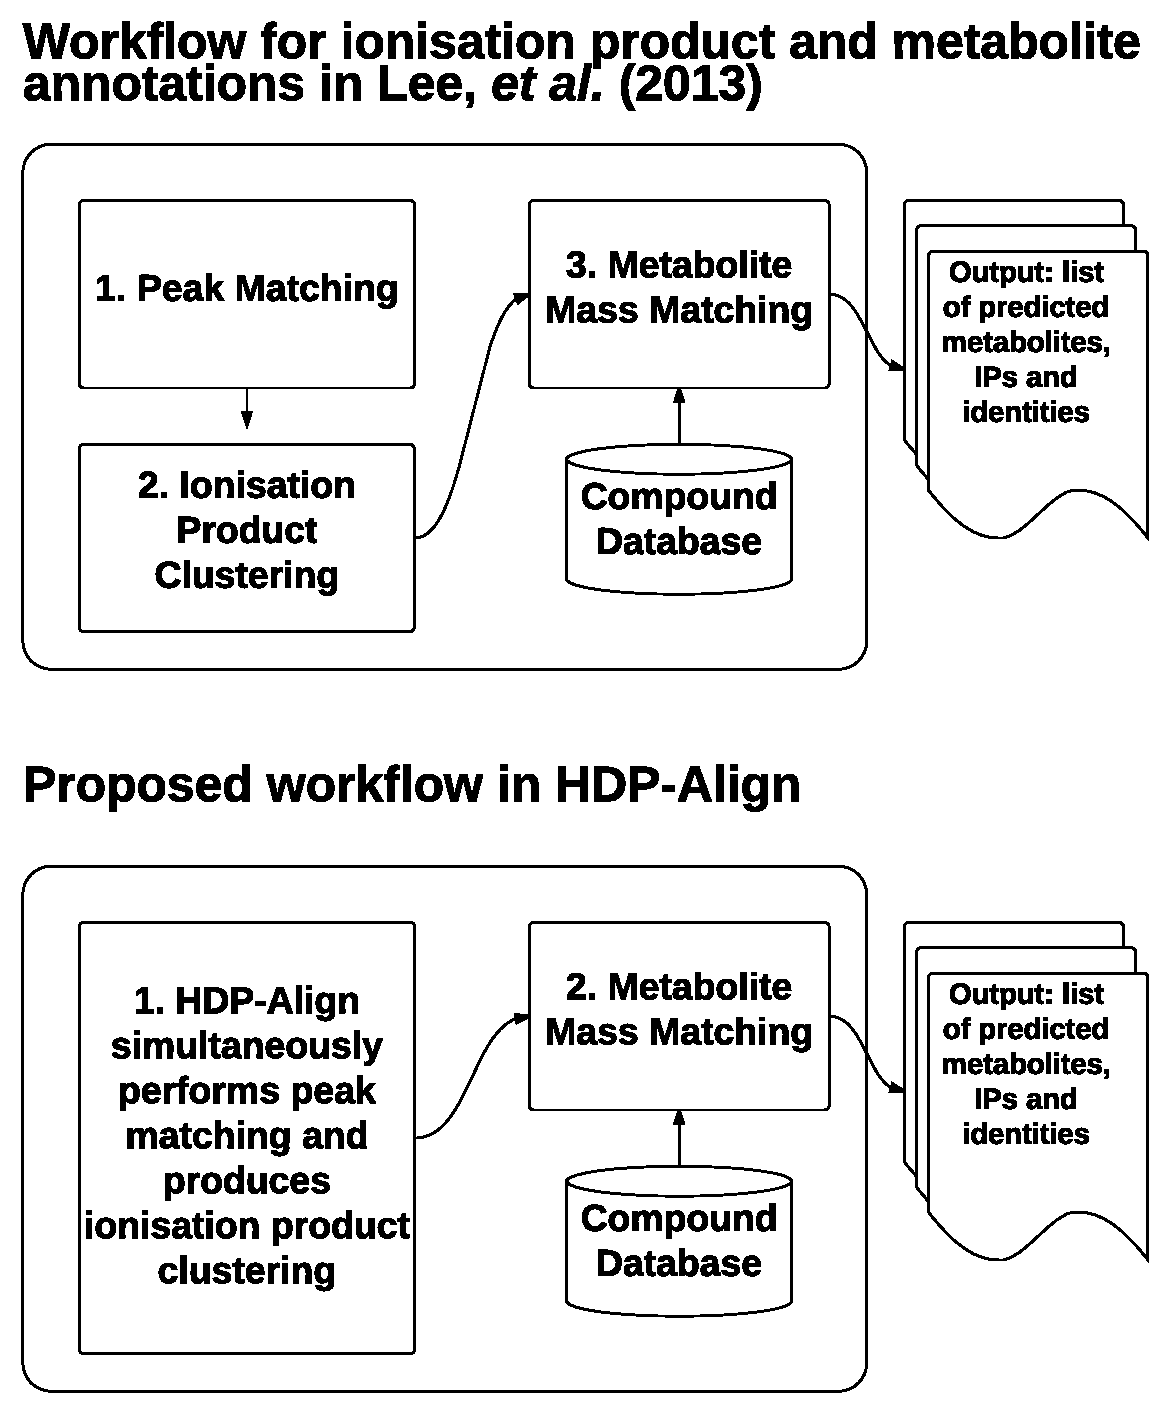
\includegraphics[width=0.5\linewidth]{06-hdp/figures/figure_3.eps}
\centering\caption{Comparisons on the workflow to assign putative annotations on isotopic products and metabolites described in Lee. \textit{et al.} (2013) \cite{Lee2013} and in HDP-Align.\label{fig-workflow}}
\end{figure}

\section{Evaluation Study}

\subsection{Evaluation Datasets}

The performance of the proposed methods and other benchmark methods is evaluated on the LC-MS datasets for the proteomic, glycomic and metabolomic experiments first introduced in Section~\ref{sub:evaluation-study}. Unlike the PrecusorCluster model in Chapter~\ref{c:precursor-clustering} that requires a list of transformation rules, defined to be specific for metabolomics in in Chapter~\ref{c:precursor-clustering}, the HDP-Align model is more flexible as it does not require such rules to group related peaks within and across runs. 

As before, all 6 fractions from the P1 Proteomic dataset in \cite{Lange2008} are used. Each fraction contains 2 runs of features having high \ac{RT} variations across runs are used in our experiments. From Section~\ref{sub:glycomic-dataset}, we use the first 10 runs of the Glycomic dataset provided by \cite{Tsai2013a} for our multiple-runs experiment. Additionally, the Standard metabolomic dataset, first introduced in Section~\ref{sub:metabolomic-dataset}, is also used. Here, we selected the first 6 out of the 11 runs for our experiment and applied an intensity threshold of 5E4 to reduce the number of features. Table~\ref{tab:hdp-datasets} summarises the different evaluation datasets and the number of features each dataset has.

\begin{table}[!htbp]
\begin{centering}
\begin{tabular}{|c|c|c|}
\hline 
Dataset & No. runs & Total Features\tabularnewline
\hline 
\hline 
P1 Frac 000 & 2 & 10606\tabularnewline
\hline 
P1 Frac 020 & 2 & 2135\tabularnewline
\hline 
P1 Frac 040 & 2 & 2188\tabularnewline
\hline 
P1 Frac 060 & 2 & 3342\tabularnewline
\hline 
P1 Frac 080 & 2 & 2086\tabularnewline
\hline 
P1 Frac 100 & 2 & 1326\tabularnewline
\hline 
Glycomic & 10 & 9344\tabularnewline
\hline 
Metabolomic & 6 & 7477\tabularnewline
\hline 
\end{tabular}
\par\end{centering}

\caption{Total number of runs and features of the selected evaluation datasets. \label{tab:hdp-datasets}}
\end{table}

\subsection{Baseline Methods for Evaluation}

Alignment performance is evaluated following the definition of precision and recall in Section~\ref{sub:Performance-Measures}. To summarise, every alignment method return a list of aligned peaksets. Each aligned peakset can be broken into all the possible $l$-size combinations of peaks in the peakset, with each combination constituting an alignment item. From a method we obtain the set of alignment items, $M$, while from the ground truth, we obtain the set of alignment items $G$. True Positives ($\boldsymbol{TP}$) are items that should be matched (in $G$) and are actually matched (in $M$). False Positives ($\boldsymbol{FP}$) are items that should not be matched (not in $G$) but are matched (in $M$), while False Negatives ($\boldsymbol{FN}$) are items that should be matched (in $G$) but are not matched (in $M$). A method with a perfect alignment output would have both precision and recall values of 1.0. 

Following Chapter~\ref{c:matching}, we benchmark HDP-Align against two established alignment methods: SIMA \cite{Voss2011a} and MZmine2's Join Aligner \cite{Pluskal2010}. The selection of SIMA and Join as the baseline methods is motivated by the fact that both methods are direct matching methods (thus easily comparable to HDP-Align) that work on generally any LC-MS-based omics data. They also sufficiently differ in how they establish the final alignment results, in particular when it comes to the alignment of multiple runs. This is primarily due to the differences between both methods in the form of the distance/similarity function between peaks, the actual matching algorithm itself and the merging order of pairwise results to construct the full alignment results. The two most important parameters to configure in the baseline methods are the mass and \ac{RT} tolerance parameters, used for thresholding and computing feature similarities during matching. We label these common parameters as the $T_{(m/z)}$ and $T_{rt}$ parameters. Note that despite the common label, each method may use the parameter values differently during the alignment process. In our experiments, we let $T_{(m/z)}$ and $T_{rt}$ vary within reasonable ranges (details in Section~\ref{sub:parameter-optimisations}) and report all performance values generated by each combination of the two parameters.

\subsection{Parameter Optimisations}
\label{sub:parameter-optimisations}

Tables~\ref{tab:hdp-parameters-hdpalign} and ~\ref{tab:hdp-parameters-benchmark} describe the parameter ranges of each method during performance evaluation. For HDP-Align (Table~\ref{tab:hdp-parameters-hdpalign}), we perform the experiments based on our initial choices on the appropriate parameter values. These are almost certainly less than optimal and can be optimised further. The mass cluster standard deviation $\sqrt{\rho^{-1}}$ for HDP-ALign is set to the equivalent value in parts-per-million (ppm). These are 500 ppm for the Proteomic dataset and 3 ppm for the Glycomic and Metabolomic datasets. The local (within-run) cluster \ac{RT} standard deviation $\sqrt{\gamma^{-1}}$ is assumed to be fairly constant and set to 2 seconds for all datasets, while the global cluster standard deviation $\sqrt{\delta^{-1}}$ is set in the following dataset-specific manner: 50 seconds for the Proteomic dataset and 20 seconds for the remaining datasets. The larger standard deviation value is required for the Proteomic dataset to accomodate for greater \ac{RT} drifts across runs. Other hyperparameters in HDP-Align are fixed to the following values: $\alpha'=10$, $\alpha_t=10$, $\alpha_m=100$. The values of the precision hyperparameters for global cluster RT ($\sigma_0$) and mass cluster ($\rho_0$) are set to a broad value of 1/5E6. No significant changes were found to the results when these hyperparameters for the DP concentrations and cluster precisions were varied. The mean hyperparameters $\mu_0$ and $\psi_0$ are set to the means of the RT and m/z values of the input data respectively. During inference, 10000 posterior samples were obtained with the first 5000 used as burn-in, and taking every 10-th sample after burn-in for the posterior probabilities of peaks to be matched.

\begin{table}[!htbp]
\begin{centering}
\begin{tabular}{|c|c|}
\hline 
Dataset & HDP\tabularnewline
\hline 
\hline 
P1 Frac 000 & \multirow{6}{*}{$\sqrt{\rho^{-1}}=500$ ppm, $\sqrt{\gamma^{-1}}=2$ s, $\sqrt{\delta^{-1}}=50$
s}\tabularnewline
\cline{1-1} 
P1 Frac 020 & \tabularnewline
\cline{1-1} 
P1 Frac 040 & \tabularnewline
\cline{1-1} 
P1 Frac 060 & \tabularnewline
\cline{1-1} 
P1 Frac 080 & \tabularnewline
\cline{1-1} 
P1 Frac 100 & \tabularnewline
\hline 
Glycomic & $\sqrt{\rho^{-1}}=3$ ppm, $\sqrt{\gamma^{-1}}=2$ s, $\sqrt{\delta^{-1}}=20$
s\tabularnewline
\hline 
Metabolomic & $\sqrt{\rho^{-1}}=3$ ppm, $\sqrt{\gamma^{-1}}=2$ s, $\sqrt{\delta^{-1}}=20$
s\tabularnewline
\hline 
\end{tabular}
\par\end{centering}
\caption{Parameters used for HDP-Align\label{tab:hdp-parameters-hdpalign}}
\end{table}

For SIMA and Join, we report the results from all combinations of the mass and RT tolerance parameters within reasonable ranges listed in Table~\ref{tab:hdp-parameters-benchmark}. This follows from the range of parameters selected for evaluation experiments in the previous Chapter~\ref{c:matching}. The ranges of $T_{(m/z)}$ and $T_{rt}$ parameters used are based values reported on \cite{Lange2008} for the Proteomic dataset and \cite{Tsai2013a} for the Glycomic dataset. For the Metabolomic dataset, they were chosen in light of the mass accuracy and RT deviations of the data.

\begin{table}[!htbp]
\begin{centering}
\begin{tabular}{|c|c|}
\hline 
Dataset & Benchmark (SIMA, Join)\tabularnewline
\hline 
\hline 
P1 Frac 000 & \multirow{6}{*}{$T_{(m/z)}=\{1.0,1.1,...,2.0\}$, $T{}_{rt}=\{10,20,...,180\}$ s}\tabularnewline
\cline{1-1} 
P1 Frac 020 & \tabularnewline
\cline{1-1} 
P1 Frac 040 & \tabularnewline
\cline{1-1} 
P1 Frac 060 & \tabularnewline
\cline{1-1} 
P1 Frac 080 & \tabularnewline
\cline{1-1} 
P1 Frac 100 & \tabularnewline
\hline 
Glycomic & $T_{(m/z)}=\{0.05,0.1,0.25\}$,$T{}_{rt}=\{5,10,...,120\}$ s\tabularnewline
\hline 
Metabolomic & $T_{(m/z)}=\{0.001,0.01,0.1\}$, $T{}_{rt}=\{5,10,...,120\}$ s\tabularnewline
\hline 
\end{tabular}
\par\end{centering}
\caption{Parameters used for the benchmark methods (SIMA, Join).\label{tab:hdp-parameters-benchmark}}
\end{table}

\section{Results and Discussions}

The performance of the evaluated methods methods on the different datasets are presented in Sections~\ref{sub:proteomic-results} and ~\ref{sub:glycomic-metabolomic-results}. Additionally, an example of the further annotations for the putative adduct type and metabolite identity that can be produced by HDP-Align is also shown in Section~\ref{sub:glycomic-metabolomic-results}. 

\subsection{Proteomic (P1) Results}
\label{sub:proteomic-results}

Figure~\ref{fig:proteomic_results} shows the results from performance evaluation on the Proteomic (P1) dataset. We see that both benchmark methods (SIMA and Join) produce a wide range of performance depending on the parameter values for $(T_{(m/z)}, T_{rt})$ chosen. Sensitivity to parameter values is expected on this dataset due to the low mass accuracy in the MS instrument that produces the data and the high \ac{RT} drifts present across runs (further details in \cite{Lange2008}). HDP-Align performs well on several fractions (particularly fractions 040, 060, 080, 100) with precision-recall performance close to the optimal performance attainable by the benchmark methods. On all fractions, HDP-Align is also able to produce higher-precision results compared to the benchmark methods by reducing recall through setting the appropriate values for the threshold $t$. The primary benefits of quantifying alignment uncertainties is realised here as the well-calibrated probability scores on the matching confidence of aligned peaks produced by HDP-Align allows the user to choose which point along the PR curve to operate on. It is less obvious how this can be accomplished in the benchmark methods by varying the \ac{RT} ($T_{rt}$) and m/z ($T_{m/z}$) thresholding parameters, if at all possible.

\begin{figure}[!htbp]
\centering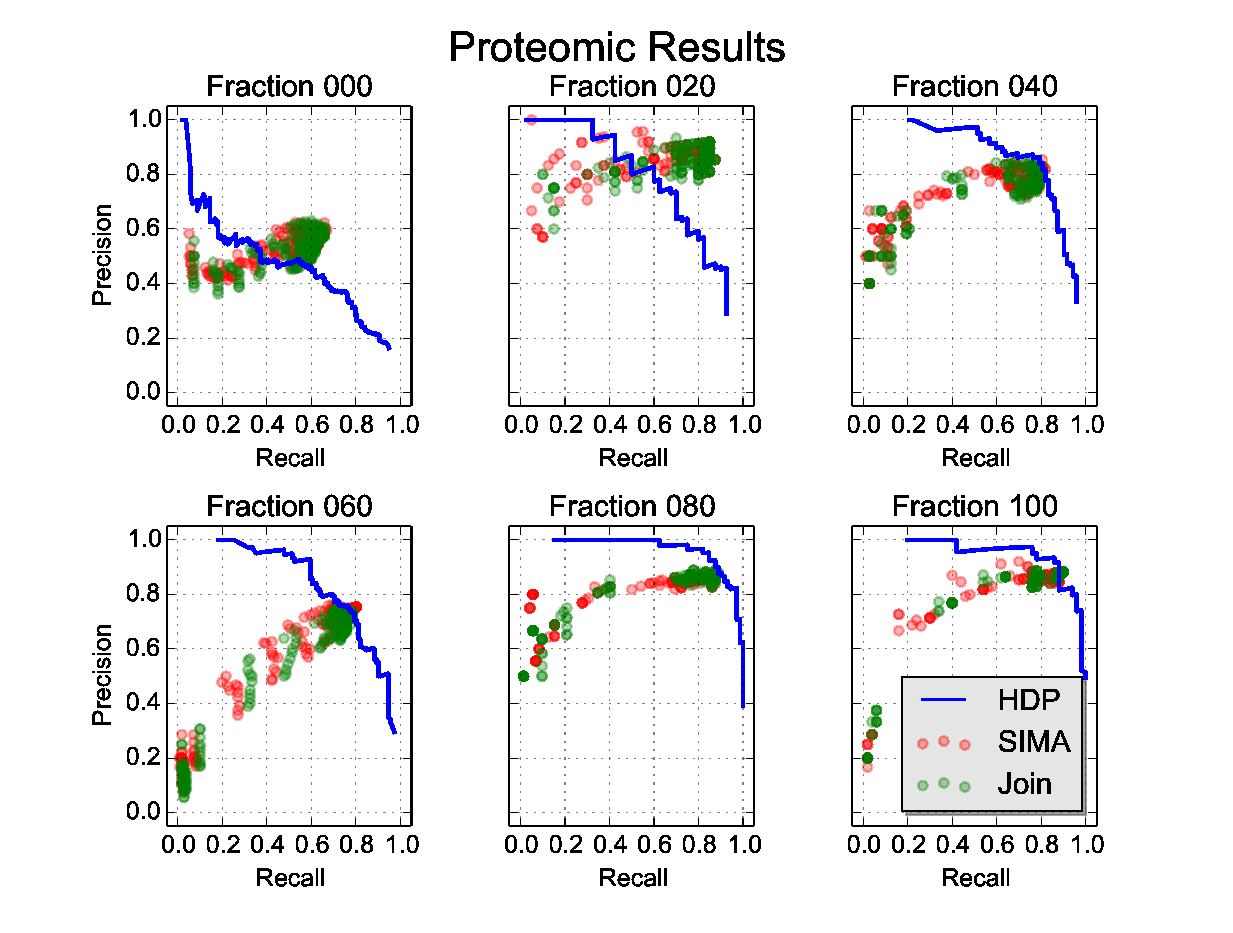
\includegraphics[width=0.7\linewidth]{06-hdp/figures/figure_4.eps}
\centering\caption{\label{fig:proteomic_results}Precision-recall values on the different fractions of the Proteomic (P1) dataset.}
\end{figure}

The P1 datasets also represent the most challenging alignment scenario as they have the largest RT drift and low mass accuracy in comparison the glycomic and metabolomic data. We use the largest (P1 Fraction 000) and the smallest (P1 Fraction 100) from P1 to examine how well our chain converges during Gibbs sampling. 

Figure~\ref{fig:traceplot_000} (left) shows the traceplots of the number of global clusters from three randomly initialised MCMC chains when running HDP-Align on the largest P1 Fraction 000 dataset containing 10606 features. From the jumps in the number of global clusters in the traceplots, we see some evidence of bad mixing in the chains. This is explained by the fact that in our sampler, we do not allow for the block reassignment of a group of peaks (that are together placed in a local cluster) into a new global cluster. Consequently, a global cluster can only be deleted when all its individual peaks have completely moved elsewhere. This leads to the slow convergence and poor mixing of the model. An inspection of the distributions of global clusters after burn-in from the three chains, shown in Figure~\ref{fig:traceplot_000} (right), also suggests that the chains have not fully converged yet. 

\begin{figure}[!htbp]
\centering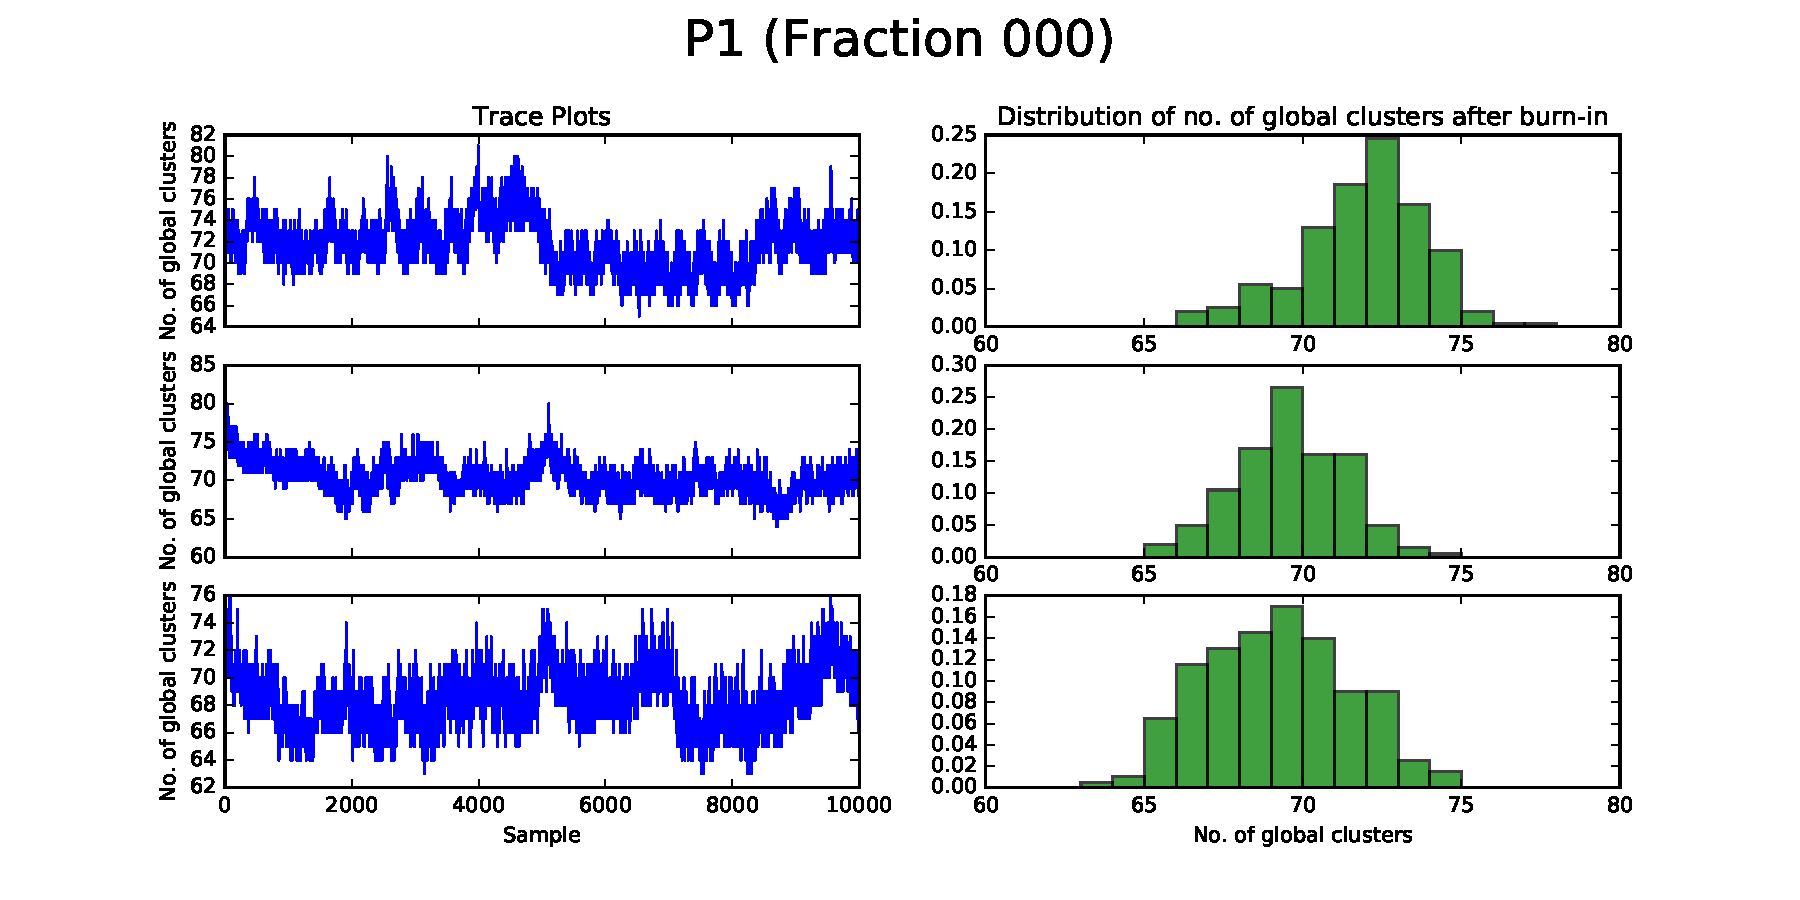
\includegraphics[width=0.7\linewidth]{06-hdp/figures/traceplot_p1_000.pdf}
\centering\caption{\label{fig:traceplot_000}Traceplots from three randomly initialised MCMC chains for the number of global clusters across all posterior samples for the largest fraction (000) from the Proteomic (P1) dataset.}
\end{figure}

Running HDP-Align on the P1 Fraction 000 data and collecting 10000 posterior samples requires several days of walltime. The main factor affecting the running time of HDP-Align is the total number of peaks across all runs to be processed and the number of samples produced during Gibbs sampling. In each iteration of Gibbs sampling, HDP-Align removes a peak from the model, updates parameters of the model conditioned on every other parameters, and reassigns a peak into RT and mass clusters. In practice, additional time will also be spent on various necessary book-keeping operations, such as deleting empty local and global clusters that are no longer required, updating internal data structures, etc. Running a longer chain may not be not entirely practical in actual analytical situation --- particularly in comparison to the speed of the baseline methods that completes in minutes. Despite this poor mixing, as the results show in Figure~\ref{fig:proteomic_results}, we still see some evidence that by reducing recall, it is still possible to extract from HDP-Align alignment results having a higher precision than what the baseline methods can achieve.

Inspecting the diagnostic plots Figure~\ref{fig:traceplot_100} for the smaller P1 Fraction 100 dataset, we observe a better mixing behaviour. The traceplots that are less jumpy and the distributions of the number of global clusters that are more consistent across the three chains. This may be due to the smaller (1326) number of features in this dataset. On this dataset, HDP-Align took two hours to process. This is a reasonable time a user can tolerate for a data analysis pipeline to complete (although still significantly longer than the baseline methods that require seconds to complete). Again from Figure~\ref{fig:proteomic_results}, the results for this P1 Fraction 100 dataset show that by trading off recall, we can obtain a higher precision than the baseline methods.

\begin{figure}[!htbp]
\centering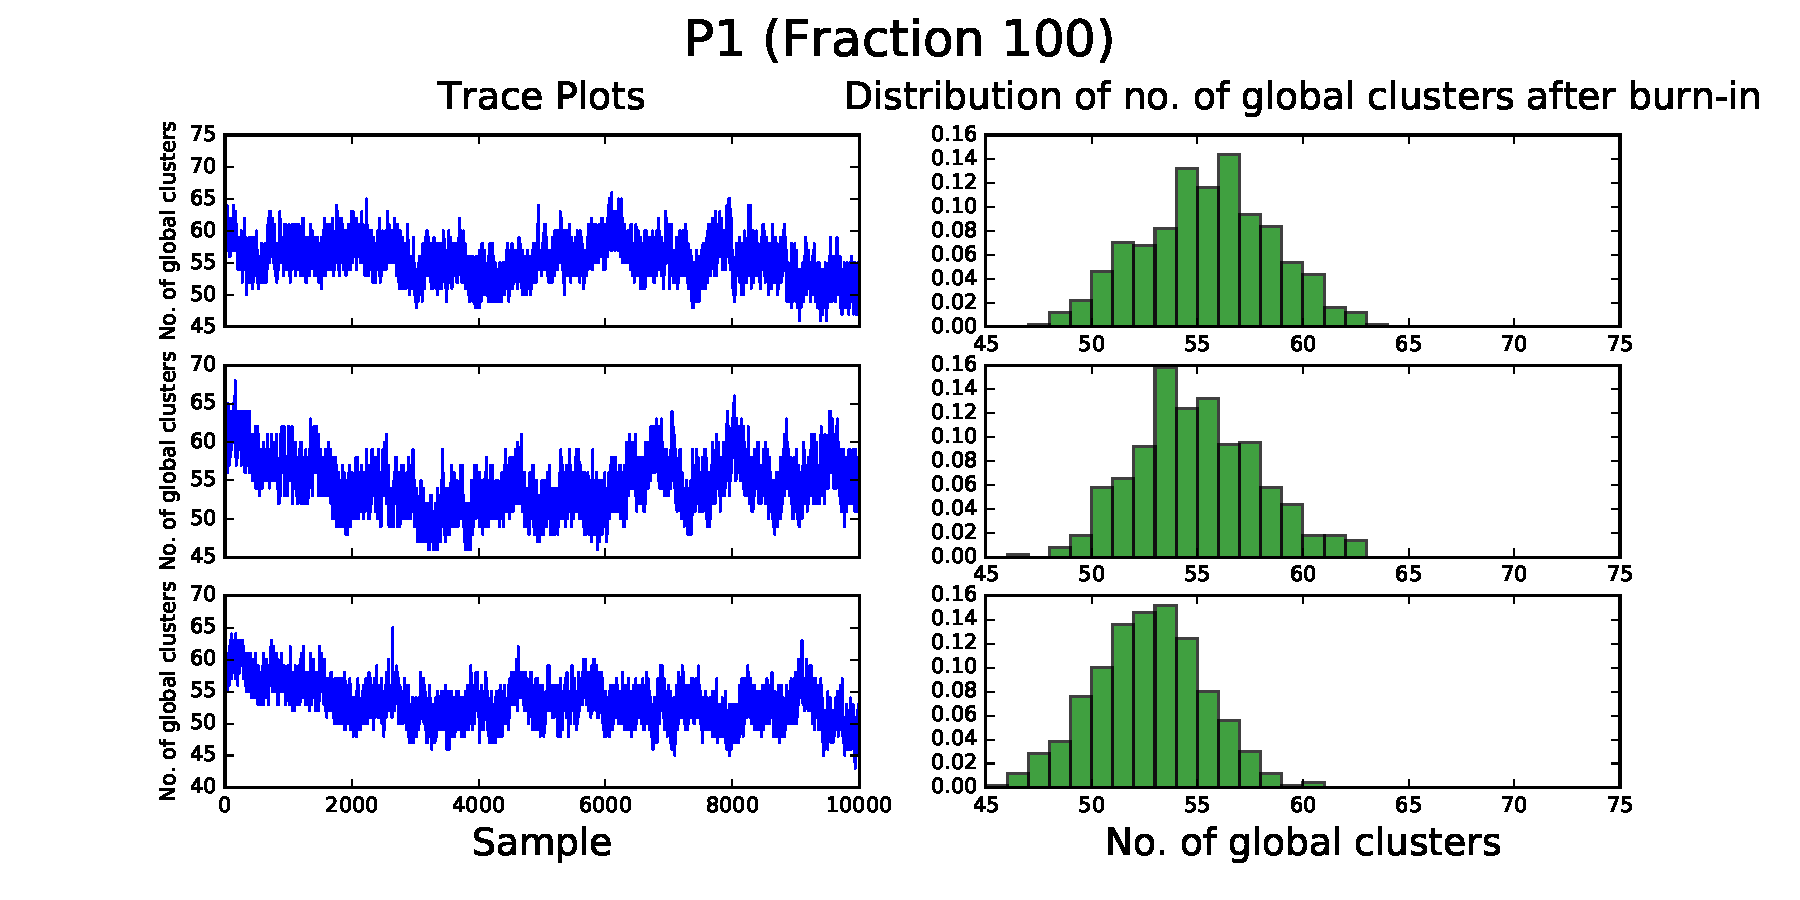
\includegraphics[width=0.7\linewidth]{06-hdp/figures/traceplot_p1_100.pdf}
\centering\caption{\label{fig:traceplot_100}Traceplots from three randomly initialised MCMC chains for the number of global clusters across all posterior samples for the smallest fraction (100) from the Proteomic (P1) dataset.}
\end{figure}

% A representative running time is given as $N=9344$ for the Glycomic dataset. HDP-Align requires approximately 5 hours to collect 1000 samples. In comparison, both SIMA and Join perform alignment within 5 to 10 seconds. Similarly, for $N=7477$ for the Metabolomic dataset, HDP-Align produces the results in approximately 4 hours after collecting 1000 samples, while SIMA and Join complete within seconds. The running time of HDP-Align, while being significantly longer than these two benchmark methods, is comparable to other computationally-intensive steps (e.g. peak detection) in a typical LC-MS pipeline.

\subsection{Glycomic and Metabolomic Results}
\label{sub:glycomic-metabolomic-results}

Figures~\ref{fig:glycomic_results} and ~\ref{fig:metabolomic_results_alignment} show the results from experiments on the Glycomic and Metabolomic datasets. Similar to the Proteomic dataset, a range of precision-recall values can be observed in the results for the benchmark methods on the two datasets. Consistent with our expectation, reducing the tolerance window on the retention time produces a smaller recall value, however this does not necessarily result in a better alignment precision. The performance of HDP-Align, using the same set of parameters on both datasets, come close to the optimal results from the benchmark methods, while still allowing the user to control the desired point along the precision-recall curve to operate on.

The results for the Glycomic dataset (Figure~\ref{fig:glycomic_results}) also show some additional results on how the measured precision-recall values might change depending on the strictness of what constitutes an alignment item during performance evaluation. This is accomplished by gradually increasing the value for $l$ that determines the size of the feature combinations enumerated from a method's output. For example, $l$=2 considers all pairwise combinations of features from the method's output during performance evaluation, while $l=4$ considers all combinations of size 4, and so on. Figure~\ref{fig:glycomic_results} shows that as $l$ is increased, parameter sensitivity seems to become more of an issue for the benchmark methods, with more parameter sets having lower precisions in the results. Across all $l$s evaluated, parameter pairs that produce the best alignment performance (points with high precision and recall values) are generally small $T_{(m/z)}$ and large $T_{rt}$ values. Examples of parameter pairs that produce the best and worse performance for SIMA are shown in Figure~\ref{fig:metabolomic_results_alignment}. The results here appear to suggest the importance of having high mass precision during matching. Importantly, we see from Figure~\ref{fig:glycomic_results} that the performance of HDP-Align remains fairly consistent as $l$ is increased.

The Metabolomic dataset also provides us with additional results in form of annotations of putative adduct type and metabolite identities. A thorough evaluation on the quality of such annotations, in comparison to e.g. the workflow proposed in \cite{Lee2013}, is beyond the scope of this chapter and would likely necessitate using a different and more appropriate evaluation dataset. Instead, we present an example of the further analysis performed by HDP-Align (as proposed in Section~\ref{subsub:isotopic-product-annotations}) on the resulting clustering objects after inference. Figure~\ref{fig:metabolomic_results_annotations} shows a global \ac{RT} cluster where peaks across runs have been grouped by their \ac{RT} and m/z values. Within this global cluster, peaks are further separated into 6 mass clusters -- corresponding to ionisation products produced by the global cluster during mass spectometry. In Figure~\ref{fig:metabolomic_results_annotations}, mass cluster $A$ and $B$ contain features aligned from several runs but they do not have any other mass cluster sharing a possible precursor mass. Mass cluster $C$ and $D$ share a common precursor mass (292.12696) and can thus be annotated by the adduct type that produce the transformation. Similarly, mass cluster $E$ and $F$ share a common precursor mass at 383.14278. Queries to a local KEGG database are issued based on the precursor mass values, producing several compound identities that can be putatively assigned to the global \ac{RT} cluster. It is a strength of the HDP-Align approach that this putative identification step appears very naturally from the alignment results.

\begin{figure}[!htbp]
\centering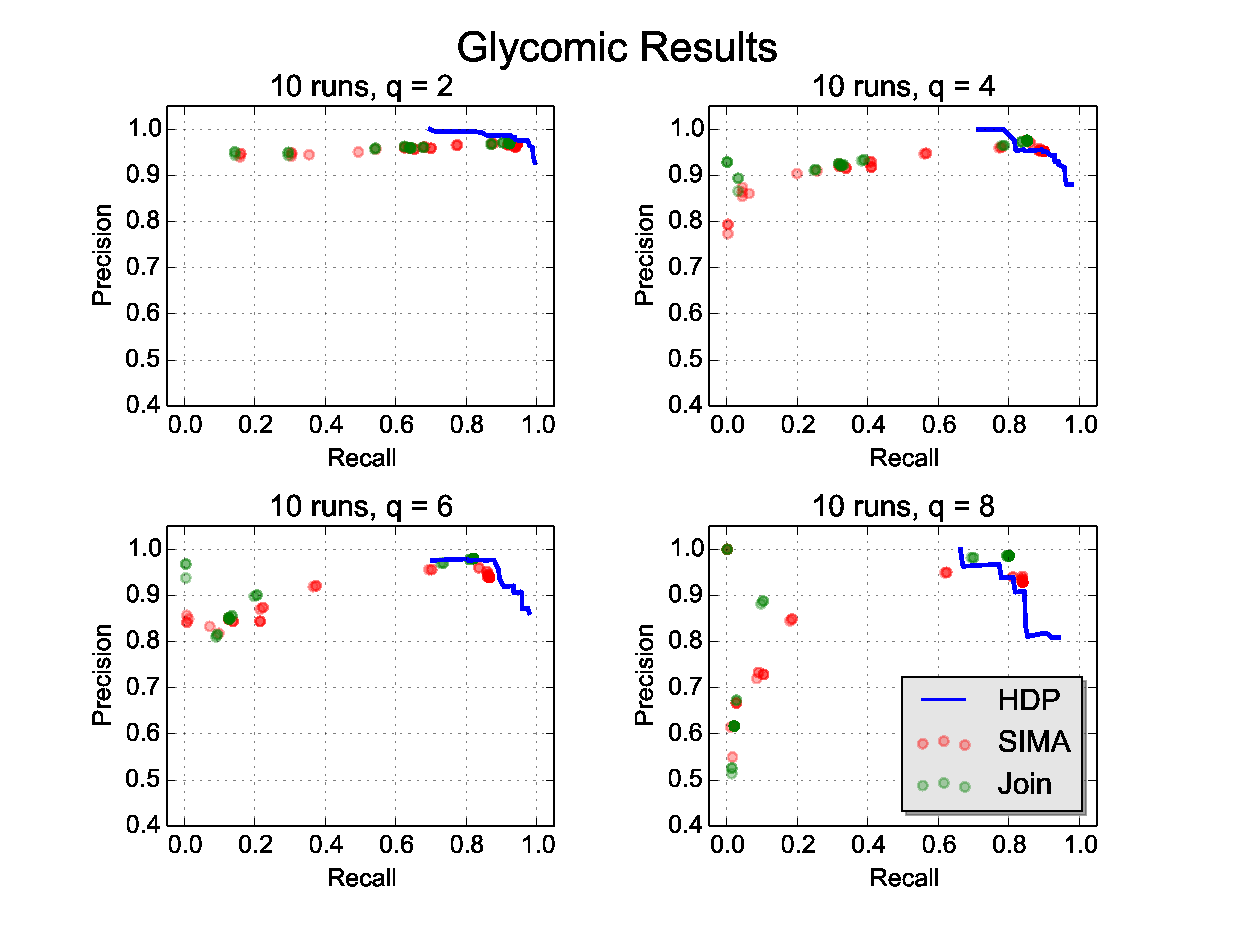
\includegraphics[width=0.7\linewidth]{06-hdp/figures/figure_5.eps}
\centering\caption{\label{fig:glycomic_results}Precision-recall values on the alignment of 10 runs from the Glycomic dataset when $q$ (the strictness of performance evaluation as described in Section~\ref{sub:Performance-Measures}) is gradually increased.}
\end{figure}

\begin{figure}[!htbp]
\centering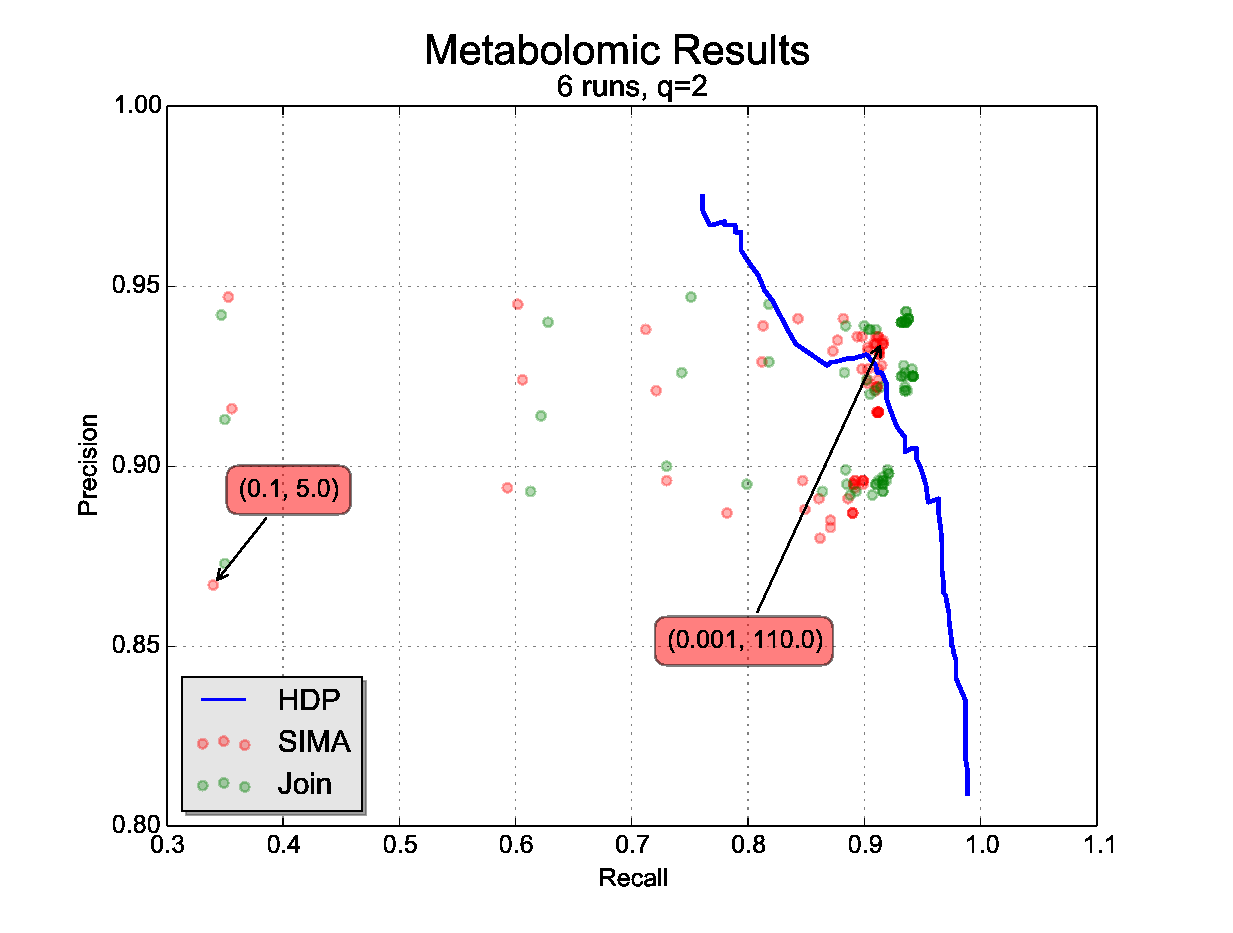
\includegraphics[width=0.7\linewidth]{06-hdp/figures/figure_6.eps}
\centering\caption{\label{fig:metabolomic_results_alignment}Precision-recall values on the alignment of 6 runs from the Metabolomic dataset. The parameter values $(T_{m/z}, T_{rt})$ that produce the best and worst performance in SIMA are also annotated in the Figure (red boxes).}
\end{figure}

\begin{figure}[!htbp]
\centering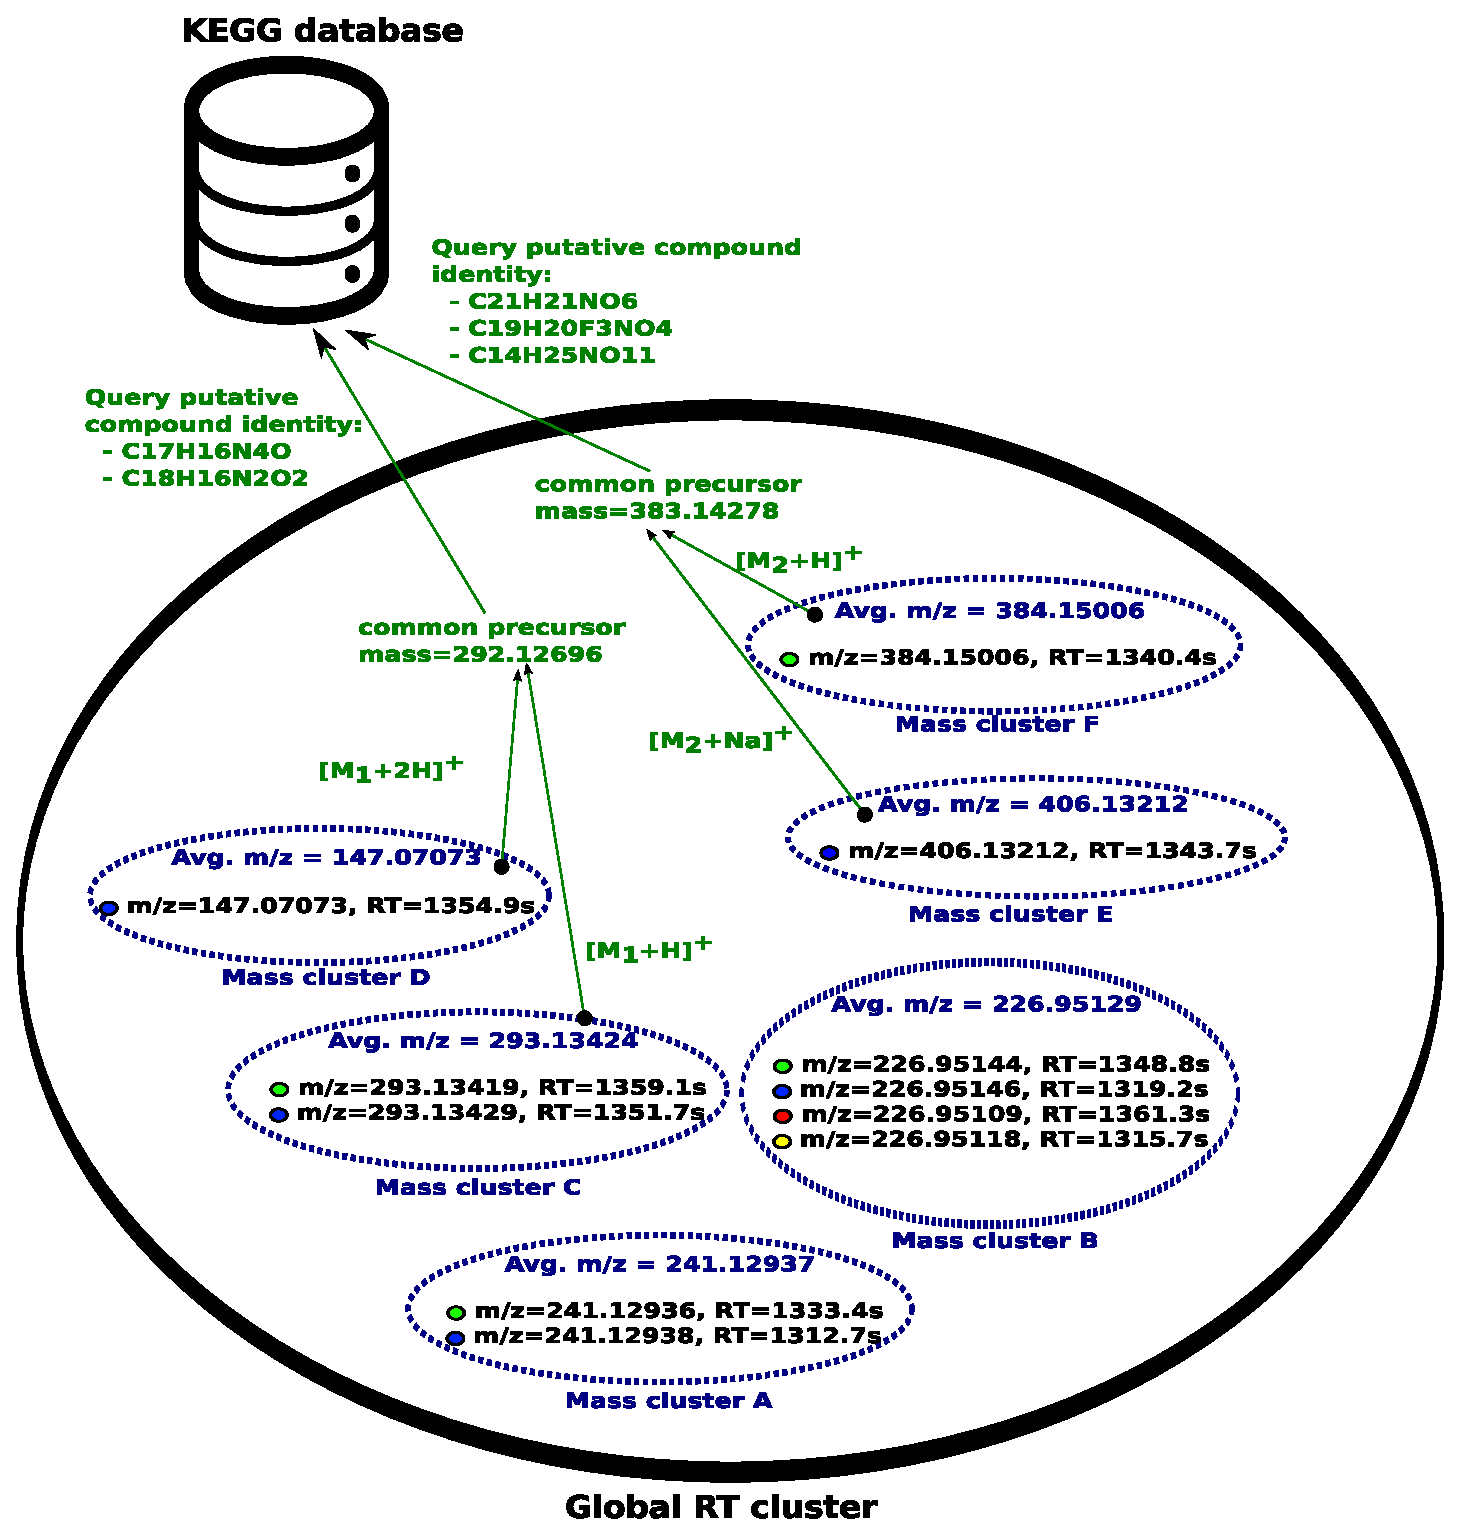
\includegraphics[width=0.7\linewidth]{06-hdp/figures/figure_7.eps}
\centering\caption[Example analysis that can be performed on the clustering objects inferred in a Gibbs sample from HDP-Align.]{\label{fig:metabolomic_results_annotations}Example analysis that can be performed on the clustering objects inferred in a Gibbs sample from HDP-Align. The outer black oval denotes a global RT cluster (generally corresponding to a metabolite compound), while the smaller dotted ovals within denote mass clusters (labelled as mass cluster $A,B,C,D,E,F$). peaks are denoted by the filled circle, with the fill colour indicating the originating run of a peak. Green colours denote additional analysis steps that can be performed on the mass cluster objects.}
\end{figure}

\section{Conclusion}

\label{sec:conc}

In this chapter, we present HDP-Align, a hierarchical non-parametric Bayesian model that simultaneously performs the within-run clustering and across-run clustering of peaks. As a natural consequence of the clustering process, the direct matching of peaks can be extracted from the model. In addition, the clustering objects from the model can also be used for further analysis in the pipeline as they potentially correspond to the actual chemical compounds that generate the generate. Similar to the two-stage clustering methods (Cluster-Cluster) introduced in the previous chapter, the HDP-Align model is able to produce well-calibrated probability scores on the matching confidence of aligned peaks (evidenced by the increasing precision and decreasing recall as the threshold $t$ is increased). This is accomplished by casting the multiple alignment problem of LC-MS peaks as a hierarchical clustering problem. Matching confidence can be obtained based on the probabilities of co-eluting peaks to be placed under the same mass component in the same global cluster. Experiments based on datasets from real proteomic, glycomic and metabolomic experiments show that HDP-Align is able to produce alignment results competitive to the benchmark direct-matching alignment methods, with the added benefit of being able to provide a measure of confidence in the alignment quality. This can be useful in real analytical situations, where neither the optimal parameters nor the alignment ground truth is known to the user.

A primary weakness of HDP-Align lies in the long computational time required to produce results. This is due to the slow mixing of the chains, as the consequence of our incremental Gibbs sampling that samples one variable at a time. The split-and-merge MCMC algorithm for the HDP proposed in \cite{Wang2012} may help to improve sampling performance and is an avenue for future work. The actual running time for the sampling can also be improved by taking the lessons from the Cluster-Cluster approach introduced in the previous chapter, for instance it may be possible to partition the data into subsets of peaks based on their retention time as only peaks within a certain RT tolerance should ever be clustered and matched to each other. The key insight of the HDP-Align model lies in the way related IP peaks are modelled as within-file clusters in a single run but the model also allows these within-file clusters to be generated by globally-shared clusters spanning multiple runs. The results presented in the current chapter suggest the method shows enough promise to warrant the effort to speed it up. 

Additional sources of information present in the LC-MS data, such as chromatographic peak shapes, can also be used to improve alignment performance and subsequent analyses that follow. The mixture of mass components used in HDP-Align with a more appropriate mass model, such as that in MetAssign \cite{Daly2014} that specifically takes into account the inter-dependency structure of peaks. Alternatively, it may be possible to build the transformation rules employed by the PrecursorCluster model (from the previous chapter) into HDP-Align. However, such modifications will introduce even more complexity to an already complex model, requiring a more sophisticated inference scheme and perhaps an even longer running time.

Through comparisons against benchmark methods, our studies have also investigated the effect of sub-optimal parameter choices on alignment performance. While beyond the scope of our paper, we agree with \cite{Smith2013, Smith2013a} that thorough investigations into the influence of numerous configurable parameters (prevalent in nearly all LC-MS data processing pipeline) on the resulting biological conclusions are of utmost importance. This should be followed by the development of methods to minimise or automatically-tune such configurable parameters. Despite the abundance of new methods proposed for LC-MS data pre-processing, relatively few studies have been done on the subject of quantifying uncertainties and alleviating the burden of parameter optimisations during actual data analysis. One way to minimise the number of parameters is through the integration of multiple steps in the typical LC-MS pipeline into fewer steps. Our proposed model in HDP-Align can potentially be extended in this manner, as evidenced by the metabolomic dataset results where we directly use the clustering objects inferred from the model to perform further analysis on putative adduct and metabolite type annotations. While the proposed annotation approach in Section~\ref{subsub:isotopic-product-annotations} is fairly simple, it can be easily extended to more sophisticated annotation strategies, such as in CAMERA \cite{Kuhl2012}. This will be particularly useful when we aim to extend the proposed model in HDP-Align into a single inferential model that encompasses many intermediate steps in a typical LC-MS data processing pipeline. 

Our experiments of taking the clustering objects from HDP-Align and using them to assign metabolite identities to the clusters through matching to a compound database also shows the potential of HDP-Align in assisting compound identification by allowing identifying labels to be assigned to a group of matched peaks from several runs at once. Identification of metabolites, particularly in large-scale untargeted experiments, is a challenging problem. In the next chapter, we propose exploiting a different kind of structural information, present in mass spectrometry fragmentation data, to aid identification.